\documentclass[]{article}
\usepackage{lmodern}
\usepackage{float}
\usepackage{amssymb,amsmath}
\usepackage{ifxetex,ifluatex}
\usepackage{fixltx2e} % provides \textsubscript
\ifnum 0\ifxetex 1\fi\ifluatex 1\fi=0 % if pdftex
  \usepackage[T1]{fontenc}
  \usepackage[utf8]{inputenc}
\else % if luatex or xelatex
  \ifxetex
    \usepackage{mathspec}
    \usepackage{xltxtra,xunicode}
  \else
    \usepackage{fontspec}
  \fi
  \defaultfontfeatures{Mapping=tex-text,Scale=MatchLowercase}
  \newcommand{\euro}{€}
\fi
% use upquote if available, for straight quotes in verbatim environments
\IfFileExists{upquote.sty}{\usepackage{upquote}}{}
% use microtype if available
\IfFileExists{microtype.sty}{%
\usepackage{microtype}
\UseMicrotypeSet[protrusion]{basicmath} % disable protrusion for tt fonts
}{}
\usepackage[margin=1in]{geometry}
\usepackage{graphicx}
\makeatletter
\def\maxwidth{\ifdim\Gin@nat@width>\linewidth\linewidth\else\Gin@nat@width\fi}
\def\maxheight{\ifdim\Gin@nat@height>\textheight\textheight\else\Gin@nat@height\fi}
\makeatother
% Scale images if necessary, so that they will not overflow the page
% margins by default, and it is still possible to overwrite the defaults
% using explicit options in \includegraphics[width, height, ...]{}
\setkeys{Gin}{width=\maxwidth,height=\maxheight,keepaspectratio}
\ifxetex
  \usepackage[setpagesize=false, % page size defined by xetex
              unicode=false, % unicode breaks when used with xetex
              xetex]{hyperref}
\else
  \usepackage[unicode=true]{hyperref}
\fi
\hypersetup{breaklinks=true,
            bookmarks=true,
            pdfauthor={Yida Yin},
            pdftitle={Data for Diplomas},
            colorlinks=true,
            citecolor=blue,
            urlcolor=blue,
            linkcolor=magenta,
            pdfborder={0 0 0}}
\urlstyle{same}  % don't use monospace font for urls
\setlength{\parindent}{0pt}
\setlength{\parskip}{6pt plus 2pt minus 1pt}
\setlength{\emergencystretch}{3em}  % prevent overfull lines
\setcounter{secnumdepth}{0}

%%% Use protect on footnotes to avoid problems with footnotes in titles
\let\rmarkdownfootnote\footnote%
\def\footnote{\protect\rmarkdownfootnote}

%%% Change title format to be more compact
\usepackage{titling}

% Create subtitle command for use in maketitle
\newcommand{\subtitle}[1]{
  \posttitle{
    \begin{center}\large#1\end{center}
    }
}

\setlength{\droptitle}{-2em}
  \title{Data for Diplomas}
  \pretitle{\vspace{\droptitle}\centering\huge}
  \posttitle{\par}
  \author{Yida Yin}
  \preauthor{\centering\large\emph}
  \postauthor{\par}
  \date{}
  \predate{}\postdate{}



\begin{document}

\maketitle


\section{Introduction}\label{introduction}

The 2015 `Data for Diplomas' run by AT\&T provides a rich dataset with
detailed information of high school graduation rates between races. The
goal of this competation is trying to help increase U.S. high school
graduation rates to 90\% by the year 2020.

Do people of different races have different performance? Does financial
condition of the family have an effect on the graduation rate? And
finally trying to discover how to increase the high school graduation
rate?

To answer these questions, I used GUIDE to choose some important
variables and visualize them to see if any patterns emerge. After that I
constructed a tree model to find out how these factors will affect the
graduation rate and then I attempted to explain the model. In this
report, I'm not trying to fit a model and give a prediction to the
graduation rate. Instead, I want to find out what are the important
factors which will affect the graduation rate.

\subsection{Data Manipulation}\label{data-manipulation}

First, we need to manipulate the data to make it easier to deal with.
The five things I have done are listed below:

\paragraph{1.Convert empty string to
NA}\label{convert-empty-string-to-na}

Since there are many empty strings in the data, the first thing we need
to do is to change them into NA.

\paragraph{2.Cut those variables represant `rates' into
levels}\label{cut-those-variables-represant-rates-into-levels}

Then I noticed that those ``rates'' are displayed in percentile levels
(string), so I wrote a function that returns the number (numeric)
corresponding to percentile levels. For example, if the original rates
is ``55-59'' then I choose 57 as its new value.

\paragraph{3.Remove dollar signs}\label{remove-dollar-signs}

After that, I removed the dollar signs (\$) and commas (which represent
thousands and millions)

\paragraph{4.Delete colunms which have too many
levels}\label{delete-colunms-which-have-too-many-levels}

Variables with too many levels may cause problems in building the model.
They usually contribute little to the analysis. So I deleted ``leanm11''
and ``School.District'' which are used to identify the location of
education agencies in district scale.

\paragraph{5.Delete duplicated columns}\label{delete-duplicated-columns}

There are some columns which represant the same thing, but many have
different column names. For example STNAM \& State\_name are both
``State Names'' and County \& County.1 \& County.name are all ``County
names''. For these columns, I only kept one of them and then delete all
of the others.

\subsection{Catch a Glimpse of the
Data}\label{catch-a-glimpse-of-the-data}

\subsubsection{Missing Values}\label{missing-values}

Let's take a glance at the missing values in the first file (graduation
rates). As we can see, there are more than half values missing in
``MAM\_RATE\_1112'' and ``MTR\_RATE\_1112''. So let's exclude them from
the dataset.

\begin{verbatim}

 Missings in variables:
        Variable Count
 MAM_COHORT_1112  6114
 MAS_COHORT_1112  4771
 MBL_COHORT_1112  3623
 MHI_COHORT_1112  2674
 MTR_COHORT_1112  5750
 MWH_COHORT_1112   125
 CWD_COHORT_1112   347
 ECD_COHORT_1112   157
 LEP_COHORT_1112  5304
\end{verbatim}

\subsubsection{How many are they?}\label{how-many-are-they}

Here I wanted to see and compare the number of Asian, Black, Hispanic,
White students. I also wanted to see the number of disabled and
economically disadvantaged students.

\begin{figure}[H]
\centering
\includegraphics{hw02_files/figure-latex/unnamed-chunk-7-1.pdf}
\caption{}
\end{figure}

Figure 1: MAS:Asian/Pacific Islander students; MBL:Black students; MHI:Hispanic
students; MWH:White students; CWD:children with disabilities;
ECD:economically disadvantaged students;

\subsection{Build the Model}\label{build-the-model}

Next, I began building the model and took ``ALL\_ RATE\_1112'' as my
response variable. The main algorithm I used is the GUIDE algorithm.
Before I began building the model, I first did some variable selection.

\subsection{Lesso For Variable
Selection}\label{lesso-for-variable-selection}

Our dataset contains nearly 600 variables which is a heavy burden even
for GUIDE. So before I ran GUIDE, I decided to reduce the dimension of
the dataset, i.e.~to select some important variables. The method I used
for selection is named Lasso.

Since Lasso can only handle the numeric variables, I had to exclude all
those ``Categorical variables'' in my model. Luckily, there are only two
``Categorical variables'': County\_name and STNAM(State name). I deleted
them and then run Lasso.

I chose the lambda based on the Mean Squared Error using cross
validation. The model which has the smallest mean squared error contains
about 150 variables.

\subsection{GUIDE TREE ALGORITHM}\label{guide-tree-algorithm}

Then I attempted to use GUIDE to construct a tree model. First I needed
to create a `Description file'. Please remember that we need to remove
those `rate' variables because it does not make sense to use `The
graduation rate of white students' to predict `All graduation rate'
since there is the possibility that 80\% of the students in high school
are white. The only data we can use to build the model is the census
data.

\subsection{GUIDE RESULTS}\label{guide-results}

\subsubsection{GUIDE Importance
Analysis}\label{guide-importance-analysis}

The GUIDE algorithm provides us a chance to see the importance rank of
all variables(Fig. 2). Some most important variables are listed below.

\begin{figure}[H]
\centering
\includegraphics{hw02_files/figure-latex/unnamed-chunk-11-1.pdf}
\caption{}
\end{figure}

I checked the meaning of every variable in this table and find that they
can be divided into groups. And then I took a further look at the data
based on these groups.

1: The most important variable is ``STNAM'' which stands for the state
name. Also ``County\_ name'' and ``LAND\_ AREA'' are variables which
related to location. This gives us an intuitive feeling that the
graduation rate may be largely affected by the location.

2: ``Aggregate\_ HH\_ INC\_ ACS'' ,``pct\_ Prs\_ Blw\_ Pov\_ Lev\_'' and
``Med\_ HHD\_ Inc\_ ACS\_ 08\_ 1'' measure how rich the family is.

3: ``NH\_ White\_ alone\_ CEN\_ 2'' measures the number of white people.

\paragraph{Which states are these?}\label{which-states-are-these}

It seems that the state is the most important factor, so I am curious to
know which states have the highest graduation rate. Thus, I drew a
picture below.

\begin{figure}[H]
\centering
\includegraphics{hw02_files/figure-latex/unnamed-chunk-13-1.pdf}
\caption{}
\end{figure}

Figure 3: From the map above we can see that high school graduation rates vary by
state. In general, those students who come from the north eastern
portion of the country perform better. And the graduation rate is low in
the west expect for California.

\subsubsection{What are the differences in graduation rates between
different
races?}\label{what-are-the-differences-in-graduation-rates-between-different-races}


\begin{figure}[H]
\centering
\includegraphics{hw02_files/figure-latex/unnamed-chunk-15-1.pdf}
\caption{}
\end{figure}

ECD: economically disadvantaged

Figure 4: As we can see, most of the students are white people. Within this plot
the white students tend to perform better than others. Also, those
economically disadvantaged students are more likely to graduate from
high school.

\paragraph{How will financial conditions affect the graduation rate?
What is the interaction between household income and the rate of white
people? How do they contribute to the graduation
rate?}\label{how-will-financial-conditions-affect-the-graduation-rate-what-is-the-interaction-between-household-income-and-the-rate-of-white-people-how-do-they-contribute-to-the-graduation-rate}

.

\begin{figure}[H]
\centering
\includegraphics{hw02_files/figure-latex/unnamed-chunk-16-1.pdf}
\caption{}
\end{figure}

Figure 5: In this plot, the x-axis is the median household income and
the y-axis is the ratio of people in different races. GR stands for
graduation rate. The darker points mean higher rates of graduation. The
picture in the top left corner reveals very important information, this
being that, almost all the green points are at the bottom of this plot.
This means those schools whose students are almost all colored people
have the lowest graduation rate. The rest of the pictures shows that in
particular black students and asian/pacific islander students may have
problems in high school. However, if the white people rate is larger
than 10\%, it turns out not to be the case. The graduation rate shows no
pattern if there are at least 10\% white students in the school.

\subsubsection{GUIDE Regression Tree}\label{guide-regression-tree}

\begin{figure}[H]
\centering
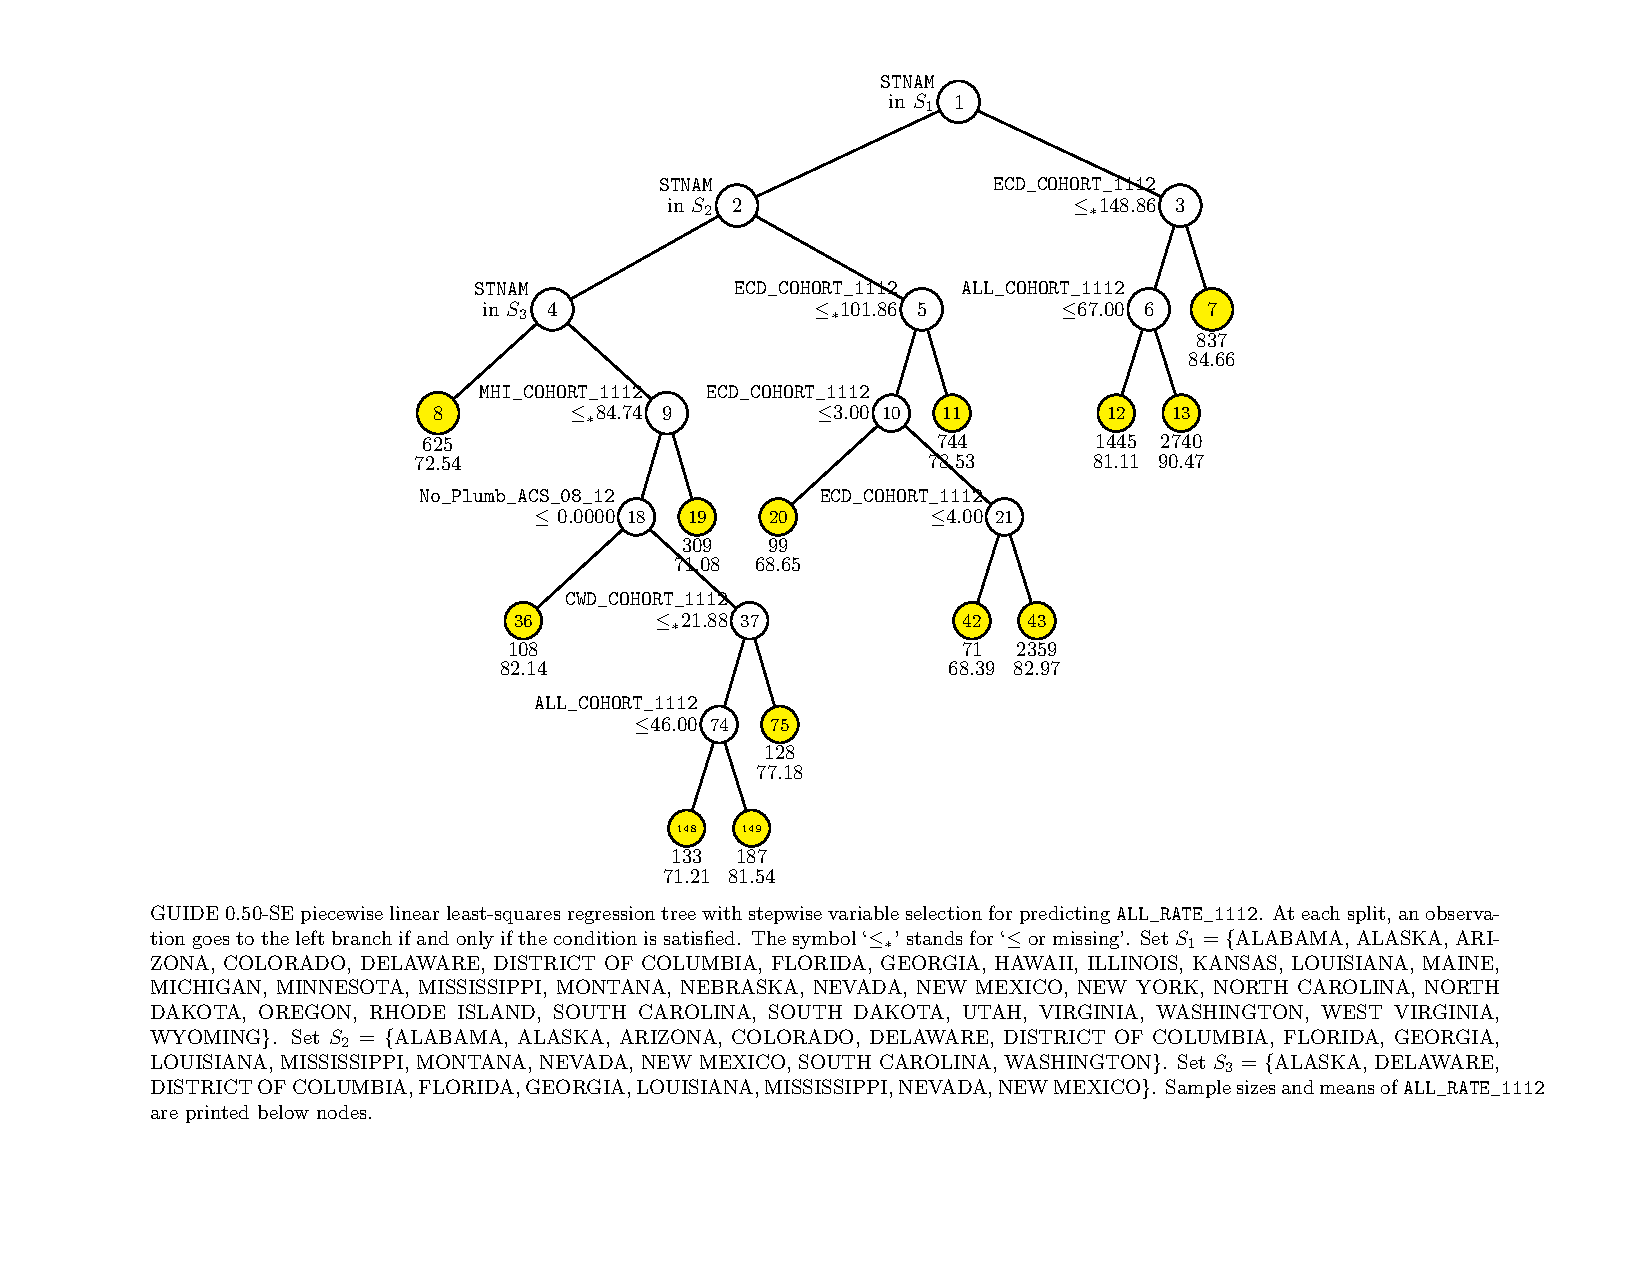
\includegraphics{hw02_files/figure-latex/tree.pdf}
\caption{}
\end{figure}

The mean squared error of this tree (Fig. 6) is 1.016E+02 while the mean squared
error of default piecewise linear least-squares regression tree is
8.507E+01. The default tree is almost the best tree we can obtain. So in
general, since their mean squared error is pretty close, this tree is
reliable. This tree fully supports my discovery above. In this tree,
``STNAM'' is the first spilt. The orange nodes on the left show the
positive relationship between white people rate/household income and
graduation rate. However, when I try to explain the right half of the
tree, I run into some trouble.  ``pct\_ Vacant\_CEN'' is something related to the census itself which is quite hard to explain; thus, within this study, we will progress past this topic.

\subsection{Conclusion}\label{conclusion}

One obvious thing we have found in this report is that high
school graduation rate varies from state to state. And in general, the
graduation rate is lower in the west. Thus, if we want to increase the
graduation rate, we must put further emphasis on the west. Another thing
is that those schools with all colored students have the lowest
graduation rate. I think it is probability because people in the same race usually live together. Schools in these districts which have a lot of colored people may not be very good. For further work, I think I need to do regression on variables "MAS\_RATE" and "MBL\_RATE". However, it is certain that we should pay more attention to those non-white students. Helping them to increase theirs graduation rate takes the first priority.
\end{document}
